\documentclass[landscape,paperwidth=42in,paperheight=52in,fontscale=0.27]{baposter} % Adjust the font scale/size here

\usepackage{graphicx} % Required for including images
\graphicspath{{figures/}} % Directory in which figures are stored

\usepackage{amsmath} % For typesetting math
\usepackage{amssymb} % Adds new symbols to be used in math mode

\usepackage{booktabs} % Top and bottom rules for tables
\usepackage{enumitem} % Used to reduce itemize/enumerate spacing
\usepackage{palatino} % Use the Palatino font
\usepackage[font=small,labelfont=bf]{caption} % Required for specifying captions to tables and figures

\usepackage{multicol} % Required for multiple columns
\setlength{\columnsep}{1.5em} % Slightly increase the space between columns
\setlength{\columnseprule}{0mm} % No horizontal rule between columns

\usepackage{tikz} % Required for flow chart
\usetikzlibrary{shapes,arrows} % Tikz libraries required for the flow chart in the template

\newcommand{\compresslist}{ % Define a command to reduce spacing within itemize/enumerate environments, this is used right after \begin{itemize} or \begin{enumerate}
\setlength{\itemsep}{1pt}
\setlength{\parskip}{0pt}
\setlength{\parsep}{0pt}
}
\renewcommand*{\thefootnote}{\Alph{footnote}}

\definecolor{lightred}{rgb}{0.698039, 0.133333, 0.133333} % Defines the color used for content box headers
\definecolor{lightblue}{rgb}{0.698039, 0.133333, 0.133333} % Defines the color used for content box headers
%\renewcommand{\thefootnote}{\arabic{footnote}}

\begin{document}

\begin{poster}
{
headerborder=closed, % Adds a border around the header of content boxes
colspacing=1em, % Column spacing
bgColorOne=white, % Background color for the gradient on the left side of the poster
bgColorTwo=white, % Background color for the gradient on the right side of the poster
borderColor=lightred, % Border color
headerColorOne=black, % Background color for the header in the content boxes (left side)
headerColorTwo=lightred, % Background color for the header in the content boxes (right side)
headerFontColor=white, % Text color for the header text in the content boxes
boxColorOne=white, % Background color of the content boxes
textborder=roundedleft, % Format of the border around content boxes, can be: none, bars, coils, triangles, rectangle, rounded, roundedsmall, roundedright or faded
eyecatcher=true, % Set to false for ignoring the left logo in the title and move the title left
headerheight=0.1\textheight, % Height of the header
headershape=roundedright, % Specify the rounded corner in the content box headers, can be: rectangle, small-rounded, roundedright, roundedleft or rounded
headerfont=\Large\bf\textsc, % Large, bold and sans serif font in the headers of content boxes
%textfont={\setlength{\parindent}{1.5em}}, % Uncomment for paragraph indentation
linewidth=2pt % Width of the border lines around content boxes
}
%----------------------------------------------------------------------------------------
%	TITLE SECTION 
%----------------------------------------------------------------------------------------
%
{
\includegraphics[height=5.5em]{mbi_logo.jpg}} % First university/lab logo on the left
{\huge\bf\textsc{Effect of Locomotion on Body Temperature Control Mechanism}} % Poster title
{\small\bf\textsc{Bohyun Kim$^1$, Yaroslav Molkov$^2$, Dmitry Zaretsky$^3$}\\
\hrulefill\\
$^1${\scriptsize Department of Mahtematics, University of California, Irvine},\\ $^2${\scriptsize Department of Mathematical Sciences, Indiana University - Purdue University Indianapolis},\\ $^3${\scriptsize Department of Emergency Medicine, Indiana University School of Medicine, Indianapolis }} % Author names and institution
{
\includegraphics[height=8.5em]{uci_logo.png}} % Sec-----ond university/lab logo on the right

%----------------------------------------------------------------------------------------
%	MOTIVATION
%-----------------------------------------------------------------------------------------

\headerbox{Motivation}{name=motivation,column=0,span = 2,row=0}{

Although humans' and other mammals' body temperature may fluctuate due to daily variation, their body temperature remain relatively constant.  However, in some cases, they experience hyperthermia despite this thermoregulatory mechanism. For instance, a stimulant such as Methamphetamine (Meth) is known to cause life-threatening hyperthermia. The injection of Meth not only causes hyperthermia but also enhances locomotion, a movement of a body, which may complicate the temperature response. The objective of this research is to observe how various intensity level of physical activities taken in different ambient temperatures affect temperature dynamics. This will allow us to analyze thermoregulatory mechanism.

\vspace{0.3em} % When there are two boxes, some whitespace may need to be added if the one on the right has more content
}

%----------------------------------------------------------------------------------------
%	CONSTRUCTING THE EXPERIMENT
%----------------------------------------------------------------------------------------

\headerbox{Constructing the Experiment}{name=experiment,column=0,span = 2, below=motivation}{ % This block's bottom aligns with the bottom of the conclusion block

A total of 32 rats were seperated into two groups of 16 rats each; one group was tested in the cool enviornment (24$^{\circ}$C) while the other group was tested in the hot environment (32$^{\circ}$C). Each group was divided into 4 subgroups depending on their exercise intensity (i.e. 4 rats in each subgroup). Over 15 mins, rats were placed in a treadmill with a speed of 0m/min, 6m/min, 12m/min, and 18m/min around either the cool or the hot enviornment. 

\begin{center}
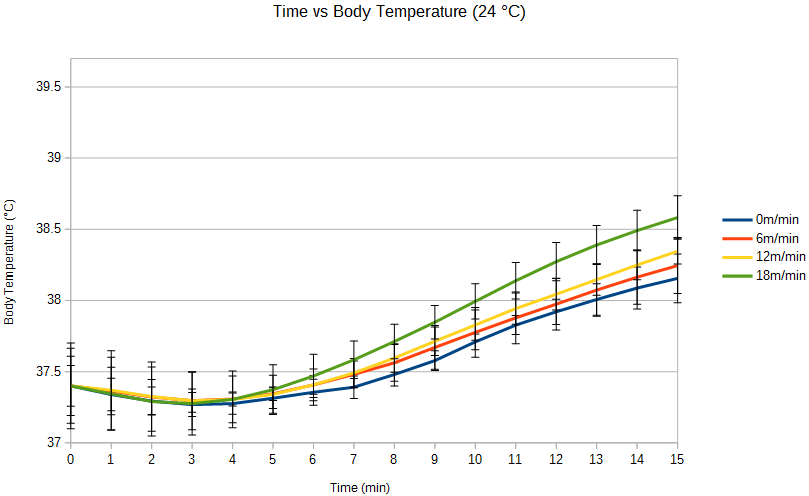
\includegraphics[width=.513\linewidth]{24deg.png}
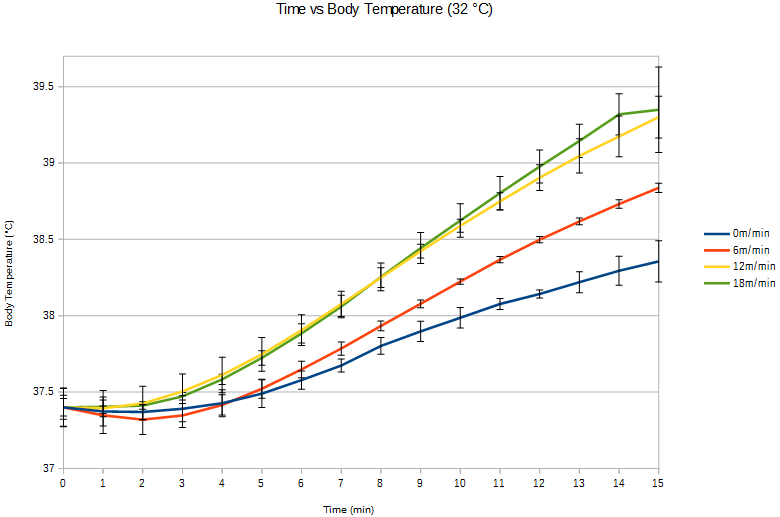
\includegraphics[width=.475\linewidth]{32deg.png}
\end{center}
\begin{itemize}\compresslist
\item We noticed the drop in temperature for 24 $^{\circ}$C and the delay in temperature rise for 32 $^{\circ}$C.
\item In 32 $^{\circ}$C, the slope of the temperature curve is more dramatic in increase of the treadmill speed than that of 24 $^{\circ}$C.
\end{itemize}
}


%----------------------------------------------------------------------------------------
%	Method
%----------------------------------------------------------------------------------------

\headerbox{Method}{name=method,column=0,span = 2, below=experiment, above = bottom}{ % This block's bottom aligns with the bottom of the conclusion block
\begin{multicols}{2}
\begin{center}
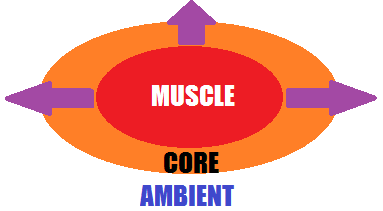
\includegraphics[width=.8\linewidth]{CORE.png}
\end{center}

\begin{itemize}\compresslist
\item Heat Dissipation from muscle to core (body) to ambient environment
\item Muscle temperature increases as body movement increases
\item Assume $\eta_{mc} = \eta_{cm}$ (i.e. the volume of muscle and the volumn of the core is the same)
\end{itemize} 
\end{multicols}

\begin{align*} 
\frac{dT_c}{dt} & = P_c - \eta_{cm} (T_c - T_m) - \eta_{ca} (T_c - T_a)\\
\frac{dT_m}{dt} & = P_m - \eta_{mc} (T_m - T_c)
\end{align*} 
\begin{itemize}\compresslist
\item $P_c$, $P_m$ : heat production of the core (body) and heat production of the muscle
\item $T_c$, $T_m$, $T_a$ : core temperature (37.4~37.5$^{\circ}$C), muscle temperature and ambient temperature (32$^{\circ}$C or 24$^{\circ}$C) 
\item $\eta_{ca}$, $\eta_{mc} = \eta_{cm}$  : heat dissipation constant between core and the ambient enviornment ($\frac{1}{50}$ in our experiment) and heat dissipation constant between core and muscle ($\frac{1}{10}$ in our experiment)
\end{itemize}

%\tikzstyle{decision} = [diamond, draw, fill=blue!20, text width=4.5em, text badly centered, node distance=2.5cm, inner sep=0pt]
\tikzstyle{block} = [rectangle, draw,  fill=red!20, text width=5em, text centered, rounded corners, node distance = 2.5cm, minimum height=5em, minimum width = 5em]
\tikzstyle{block1} = [rectangle, draw,   fill=red!20, text width=5em, text centered, rounded corners, node distance = 2.5cm, minimum height=5em]
\tikzstyle{block3} = [rectangle, draw, fill=blue!20, text width=5em, text centered, rounded corners, node distance = 2.5cm, minimum height=5em]
\tikzstyle{line} = [draw, -latex']
%\tikzstyle{cloud} = [draw, ellipse, fill=blue!20,text width=5em, text centered, node distance=5em, minimum height=2em]
\begin{center}
\begin{tikzpicture}[node distance = 2cm, auto]
\node [block] (init) {Generate Data based on Model};
\node [block1, left of=init] (Start) {Choose Pm and Pc};
%\node [cloud, right of=init] (Start2) {Start Two};
\node [block, right of=init] (init2) {Data fitting};
\node [block3, right of=init2] (End) {Analyze best fitted data};
\path [line, dashed] (init) -- (init2);
\path [line, dashed] (init2)--(init);
\path [line] (init2) -- (End);
\path [line] (Start) -- (init);
%\path [line, dashed] (Start2) -- (init);
%\path [line, dashed] (Start2) |- (init2);
\end{tikzpicture}
\end{center}
\begin{center}
\begin{tikzpicture}[node distance = 2cm, auto]
\node [block] (init) {Pm = 0.3, Pc = 0.08?};
\end{tikzpicture}
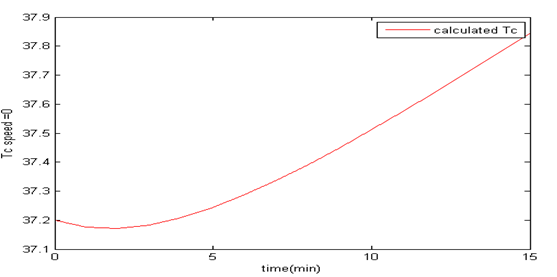
\includegraphics[width=.26\linewidth]{sample.png}
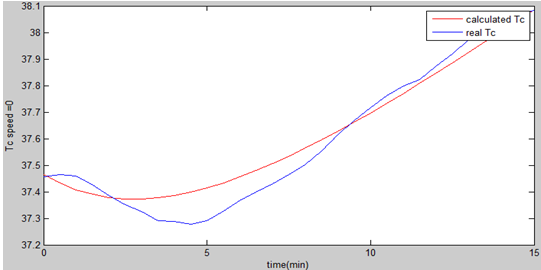
\includegraphics[width=.25\linewidth]{sample2.png}
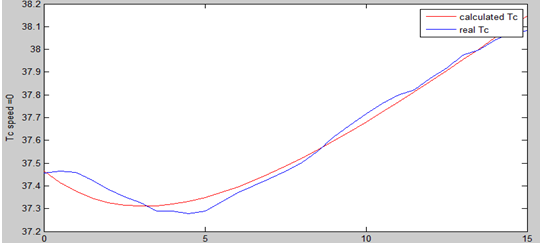
\includegraphics[width=.28\linewidth]{32best.png}
\end{center}

}

%----------------------------------------------------------------------------------------
%	RESULTS AND DISCUSSION
%----------------------------------------------------------------------------------------

\headerbox{Results and Discussion}{name=results,column=2,span=2,row=0}{
\begin{center}

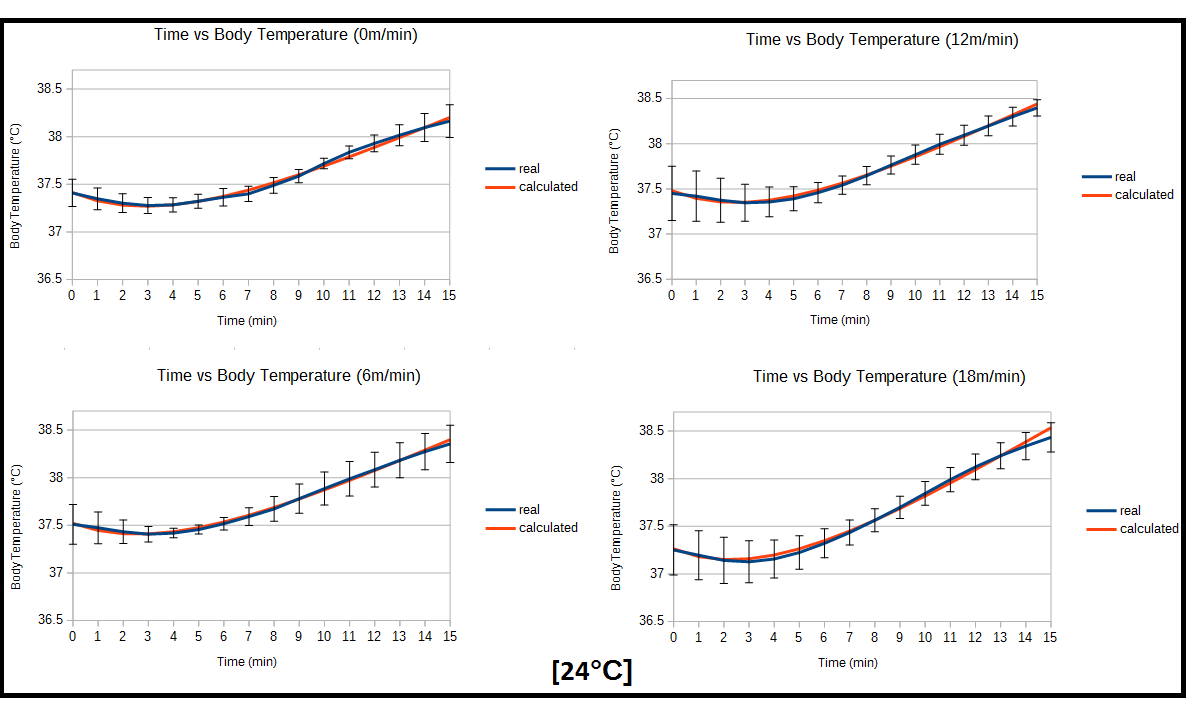
\includegraphics[width=1\linewidth]{24total.png}
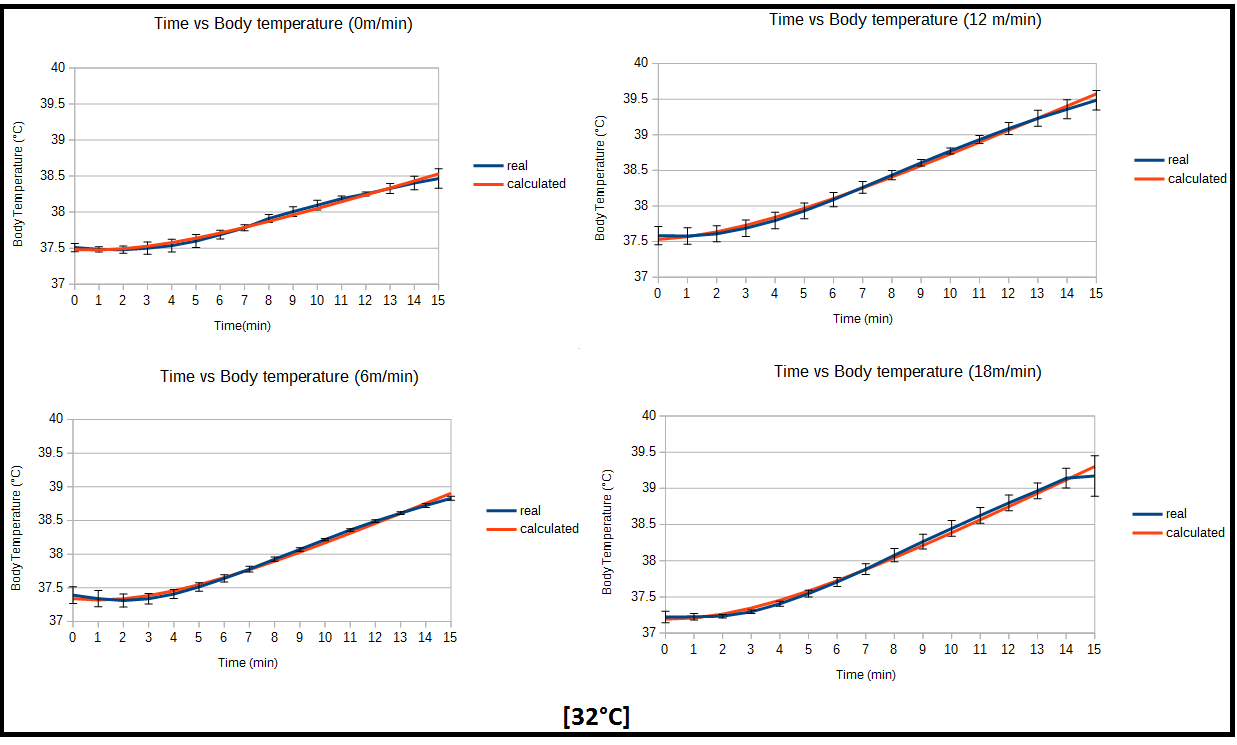
\includegraphics[width=1\linewidth]{32total.png}
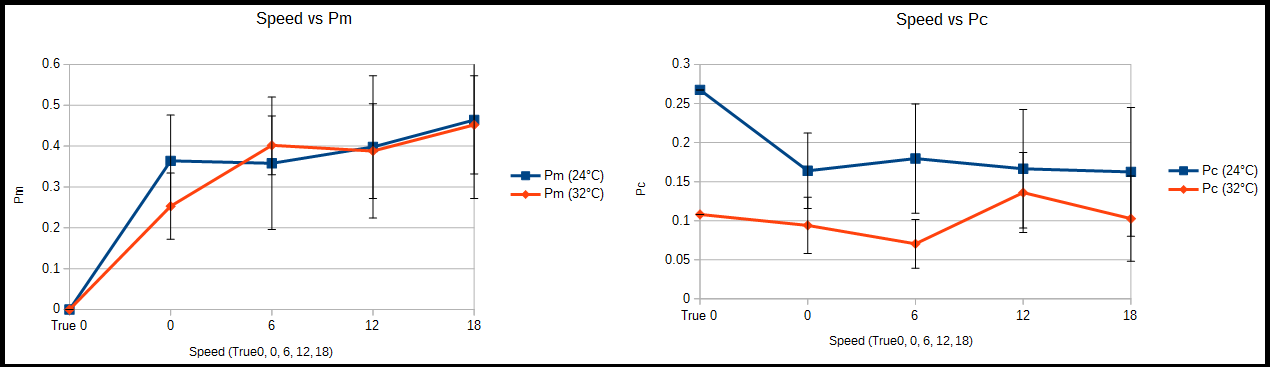
\includegraphics[width=1.001\linewidth]{pcpm.png}
\end{center}

\begin{itemize}\compresslist
\item "True 0" is when $P_{m}=0$. The respecting $Pc$ value can be calculated by setting $P_{m} = \eta_{ca} (T_c - T_a)$. 
\item We notice that $P_{m}$ dramatically increases as speed becomes True 0 to 0 m/min. This is an indication of rats body's engagement.
\item We notice that there is a significant drop in $P_{c}$ in 24 $^{\circ}$C while there is no significant drop in 32 $^{\circ}$C, $P_{c}$ when the speed varies from True 0 to 0m/min 
\end{itemize}


%\begin{multicols}{2}
%\vspace{1em}
%\begin{center}
%
\includegraphics[width=0.8\linewidth]{placeholder}
%\captionof{figure}{Figure caption}
%\end{center}

%Aliquam auctor, metus id ultrices porta, risus enim cursus sapien, quis iaculis sapien tortor sed odio. Mauris ante orci, euismod vitae tincidunt eu, porta ut neque. Aenean sapien est, viverra vel lacinia nec, venenatis eu nulla. Maecenas ut nunc nibh, et tempus libero. Aenean vitae risus ante. Pellentesque condimentum dui. Etiam sagittis purus non tellus tempor volutpat. Donec et dui non massa tristique adipiscing.
%\end{multicols}

%------------------------------------------------

%\begin{multicols}{2}
%\vspace{1em}
%Sed fringilla tempus hendrerit. Vestibulum ante ipsum primis in faucibus orci luctus et ultrices posuere cubilia Curae; Etiam ut elit sit amet metus lobortis consequat sit amet in libero. Lorem ipsum dolor sit amet, consectetur adipiscing elit. Phasellus vel sem magna. Nunc at convallis urna. isus ante. Pellentesque condimentum dui. Etiam sagittis purus non tellus tempor volutpat. Donec et dui non massa tristique adipiscing. Quisque vestibulum eros eu.

%\begin{center}
%
\includegraphics[width=0.8\linewidth]{placeholder}
%\captionof{figure}{Figure caption}
%\end{center}

%\end{multicols}
}


%----------------------------------------------------------------------------------------
%	FUTURE RESEARCH
%----------------------------------------------------------------------------------------

%\headerbox{Future Research}{name=futureresearch,column=1,span=2,aligned=references,above=bottom}{ % This block is as tall as the references block

%\begin{multicols}{2}
%Integer sed lectus vel mauris euismod suscipit. Praesent a est a est ultricies pellentesque. Donec tincidunt, nunc in feugiat varius, lectus lectus auctor lorem, egestas molestie risus erat ut nibh.

%Maecenas viverra ligula a risus blandit vel tincidunt est adipiscing. Suspendisse mollis iaculis sem, in \emph{imperdiet} orci porta vitae. Quisque id dui sed ante sollicitudin sagittis.
%\end{multicols}
%}

%----------------------------------------------------------------------------------------
%	CONTACT INFORMATION

%----------------------------------------------------------------------------------------
%	CONCLUSION
%----------------------------------------------------------------------------------------

\headerbox{Conclusion}{name=conclusion,column=2,span=2,row=0,below=results}{
\begin{itemize}\compresslist
\item We successfully showed how rats compensate their body temperature in varying ambient temperature and varying intensity of exercise.
\item In high temperature, heat production from core is maintained low attempting to maintain rats' body temperature low
\item In a room temperature, heat production from the core is maintained low as soon as rats expect locomotion. 

\end{itemize}

%------------------------------------------------


}

%----------------------------------------------------------------------------------------
%	REFERENCES
%----------------------------------------------------------------------------------------

\headerbox{References}{name=references,column=2, span = 2, below=conclusion, above=bottom}{
[1] Yaroslav, M., Maria V. Zaretskaia, and Dmitry V. Zaretsky. Meth math: modeling temperature responses to methamphetamine, \textit{Am J Physiol Regul Integ Comp Physiol.} Feb. 5, 2014. (doi:10.1152/ajpregu.00365.2013). 
}


%----------------------------------------------------------------------------------------
%	RESULTS 2
%----------------------------------------------------------------------------------------

%\headerbox{Results 2}{name=results2,column=1,below=motivation,bottomaligned=conclusion}{ % This block's bottom aligns with the bottom of the conclusion block

%Donec faucibus purus at tortor egestas eu fermentum dolor facilisis. Maecenas tempor dui eu neque fringilla rutrum. Mauris \emph{lobortis} nisl accumsan.

%\begin{center}
%\begin{tabular}{l l l}
%\toprule
%\textbf{Treatments} & \textbf{Response 1} & \textbf{Response 2}\\
%\midrule
%Treatment 1 & 0.0003262 & 0.562 \\
%Treatment 2 & 0.0015681 & 0.910 \\
%Treatment 3 & 0.0009271 & 0.296 \\
%\bottomrule
%\end{tabular}
%\captionof{table}{Table caption}
%\end{center}

%Nulla ut porttitor enim. Suspendisse venenatis dui eget eros gravida tempor. Mauris feugiat elit et augue placerat ultrices. Morbi accumsan enim nec tortor consectetur non commodo.

%\begin{center}
%\begin{tabular}{l l l}
%\toprule
%\textbf{Treatments} & \textbf{Response 1} & \textbf{Response 2}\\
%\midrule
%Treatment 1 & 0.0003262 & 0.562 \\
%Treatment 2 & 0.0015681 & 0.910 \\
%Treatment 3 & 0.0009271 & 0.296 \\
%\bottomrule
%\end{tabular}
%\captionof{table}{Table caption}
%\end{center}
%}

%----------------------------------------------------------------------------------------

\end{poster}

\end{document}